As an investigation into the utility of word vectors trained, it was decided to briefly investigate the word similarities between chemical elements. This analysis is included as an appendix as there was not sufficient space for it to be included in the main body, and due to its self-contained nature. It was hoped that this short investigation would provided evidence that methods sketched in \S\ref{sec:recomm_word_vectors} could work.

The similarity matrix was produced for chemical elements mentioned in the text corpus (115 out of 118 known chemical elements). This required mapping both chemical names and symbols together (e.g. \texttt{chlorin}\footnote{Chlorine is stemmed to chlorin by the stemming process (\S\ref{chapt:ALGORITHM}) }  and \texttt{cl} for chlorine) to represent the concept vector for the elements in question.

A modified data sanitation pipeline was created to substitute the chemical symbol for the chemical name. This was only done for chemical symbols longer than 1 letter to dissuade conflating different concepts to the same word vector (\texttt{S} could represent Sulfur or a stereochemical label.)
 
A CBOW model was trained using this modified input data with the same presets as the main CBOW model, detailed in table \ref{tab:hyperparams}. The Cosine Similarity matrix was produced for the 115 elements found in the corpus. UPGMA clustering was performed\cite{scikitlearn}, as well as graph visualisation with modularity clustering \cite{modularity1},\cite{modularity2}. The dendrogram of the UPGMA clustering is shown in figure \ref{fig:elems_dendro}. The process identified 5 main branches:
\begin{itemize}
\itemsep-0.5em
\item The gold region includes a sub-branch of noble gases, the other branch mainly actinoids.
\item The magenta region contains non-metals mostly associated with organic compounds
\item The cyan region contains mainly metalloids, actinoids and alkali metals
\item the red region contains mainly transition metals
\item The green region contains almost exclusively lanthanoid metals 
\end{itemize}
\begin{center}
\begin{figure}[H]
  \centering
    \includegraphics[width=1.2\textwidth]{Appendix/Elemental_Analysis/elements_dendro.png}
    \caption[Dendrogram for UPGMA clustering of chemical element vectors]{Dendrogram for UPGMA clustering of chemical element vectors. Colours indicate distinct branches}
    \label{fig:elems_dendro}
\end{figure} 
\end{center}
The dendrogram shows that the classifications broadly fall into intelligible categories within the periodic table. There are, however, some surprises, especially the halogens, with bromine in  the actinoid subbranch, and chlorine associating with copernicium. This may be because the symbols Cl and Cn occur together often in the literature due to mentions of carbon and nitrogen, not copernicium. Similar reasoning can be used for bromine (\texttt{cf br} could refer to a CFC rather than californium and bromine) This exposes a flaw in the symbol/name association process that could be tackled in further work.

The graph visualisation is shown in figure \ref{fig:elems_graph} (Also the front cover of this dissertation). Period 7 was removed from this graph as there were too few mentions in the corpus for reliable vectors\footnote{Uranium was kept as it had non-negligible corpus mentions}, and to remove cluttering nodes.

\begin{center}
\begin{figure}[H]
  \centering
  \textbf{Graph visualisation of chemical element vectors}
    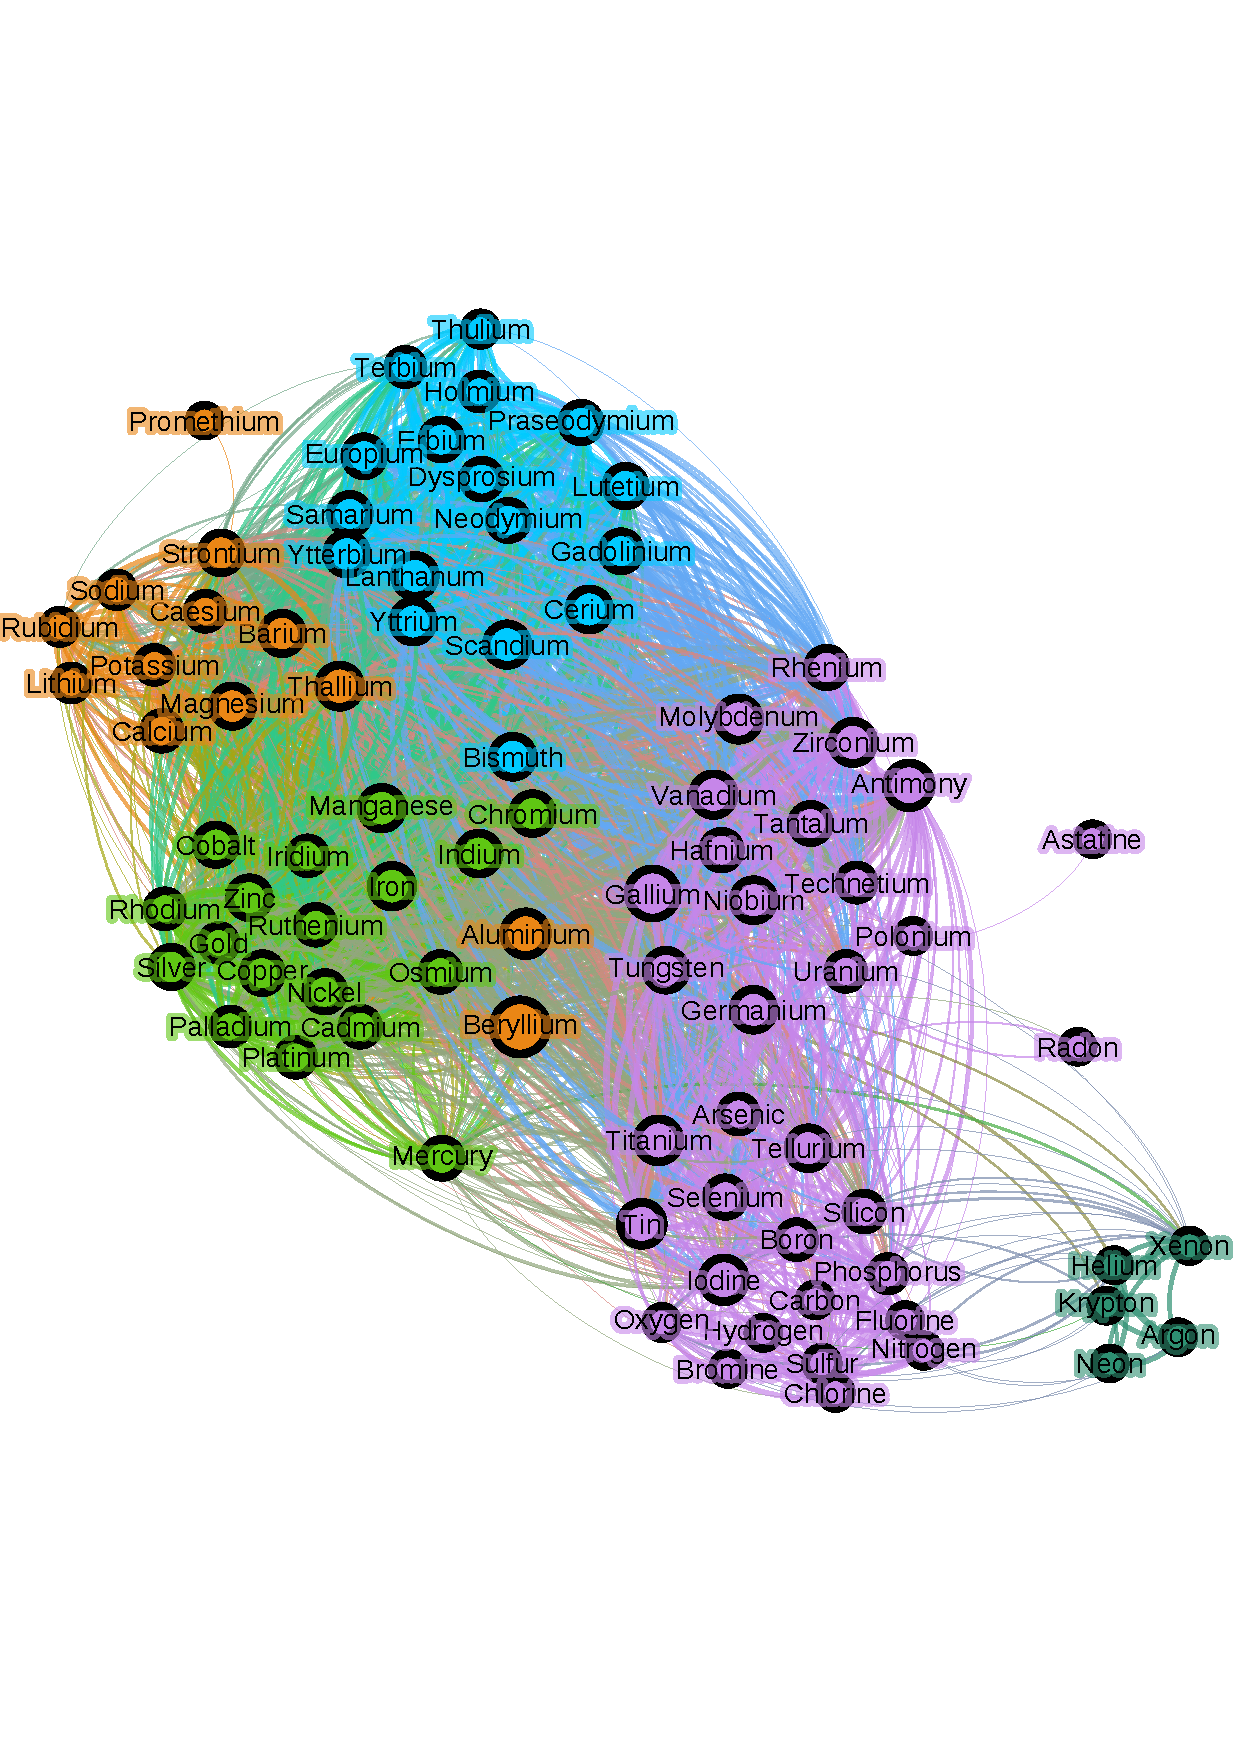
\includegraphics[width=\textwidth]{Title_Page/front_page.png}
    \caption[Graph visualisation of chemical element vectors]{Nodes are coloured by their communities, and are spatially arranged by modelling edge weights as springs. Node sizes are proportional to their connectivity. }
    \label{fig:elems_graph}
\end{figure} 
\end{center}
5 distinct communities were identified:
\begin{itemize}
\itemsep-0.5em
\item The Orange community contained mainly alkali metals and alkali earth metals
\item The Blue community contained mainly lanthanoids
\item The Light Green community contained mainly transition metals
\item The Purple community separated into two spatially distinct regions. The northern region generally contained transition metals and metalloid, and the southern region contained organic non-metals.
\item The Dark Green community contained noble gases.
\end{itemize}
The community finding process reflects a similar situation to the UPGMA process, but is perhaps more successful. The removal of the actinoids appears to have improved community finding. The community finding process was repeated with period 7 included, resulting in broadly the same communities, but with bromine and chlorine leaving the purple community to join a a loose community of actinoids, however they remained strongly associated with each other. The degree of connectivity between nodes is similar for most nodes, but larger for some nodes, e.g. beryllium, which is difficult to interpret. 

Attention was turned to a practical example. Palladium is used widely in catalysis but is rare and expensive, and alternatives would be economically and environmentally beneficial\cite{palladium}. With this in mind, the cosine similarities of all the elements to palladium vector were computed, and a selection of metallic elements with high similarity is shown in figure \ref{fig:palladium}. 
\begin{center}
\begin{figure}[H]
  \centering
  \textbf{Selected metallic elements' cosine similarity to palladium vector}
    \includegraphics[width=0.9\textwidth]{Appendix/Elemental_Analysis/metals_sorted.png}
    \caption[Selected metallic elements' cosine similarity to palladium vector]{The metals are ordered to to bottom from most similar (long bars, red) to low similarity (short bars, blue). The colours are a guide to the eye.}
    \label{fig:palladium}
\end{figure} 
\end{center}
Platinum, rhodium, ruthenium, copper and nickel all had very high scores. The models could be interpreted as suggesting that these metals have similar properties to palladium. This is very much the case for platinum and rhodium (pd, pt and rd are all platinium group metals)\cite{pgm}. Nickel and copper are predicted to be similar to palladium, and there is evidence that nickel could be used for some palladium-catalysed reactions\cite{nickel}, whereas copper is often combined with palladium to form more effective catalysts\cite{copper}. Thus it could be argued the models suggest that more attention should be focussed to nickel catalysis.

This analysis, whilst brief, is promising. This lends weight that more in-depth considerations of word vectors and concept vectors would be fruitful.